\section{Parallel Directory Structure}

\begin{itemize}
\item {\tt BoxLib/} 

 BoxLib is a library for describing meshes consisting of a union
 of boxes.  The BoxLib modules define the basic datatypes used
 in Parallel.

\item {\tt docs/}

 Documentation describing BoxLib and other directories in Parallel.

\item {\tt mglib/}

  The C++ multigrid solver.

\item {\tt mk/}

  The generic Makefiles that store the compilation flags for
  various platforms.

\item {\tt scripts/}

  Some simple scripts that are useful for building, running,
  maintaining codes in Parallel.

\end{itemize}

\section{BoxLib Data Structures}

BoxLib contains the most fundamental objects used by applications written
in the Parallel directory. The objects in BoxLib support structured
grid adaptive mesh refinement (AMR), i.e. in a single calculation
different regions of the domain can have different spatial resolutions.  
At each level of refinement, the region covered by that level is broken
into boxes, or grids.  The entire computational domain is covered by
the coarsest (base) level of refinement, often called level 0. 
Higher levels of refinement have finer zones by a ``refinement ratio''
of either 2 or 4.  Only a portion of the domain may
be covered by the higher levels of refinement.  

The grids are properly nested, in the sense that the union of grids
at level $\ell+1$ is contained in the union of grids at level $\ell$.
Furthermore, the containment is strict in the sense that,
except at physical boundaries,
the level $\ell$ grids are large enough to guarantee that there is
a border at least $n_{\rm proper}$ level $\ell$ cells wide surrounding each level
$\ell +1$ grid (grids at all levels are allowed to extend to the physical
boundaries so the proper nesting is not strict there).
For parallel computations, the boxes are distributed to processors, in
a fashion designed to put roughly equal amounts of work on each
processor (load balancing).

On a grid, the data can be stored at cell-centers, on a face/edge, or
on the corners.  In BoxLib, data that is on an edge is termed `nodal'
in that direction (see Figure~\ref{fig:dataloc}).  Data that is on the
corners is nodal in all spatial directions.  In our Parallel applications, 
the state data (velocity, density, species $\ldots$) is generally
cell-centered.  Fluxes are nodal in the direction they represent.
A few quantities are nodal in all directions (e.g.\ the pressure in
the low Mach number projection methods).

\begin{figure}[h]
\centering
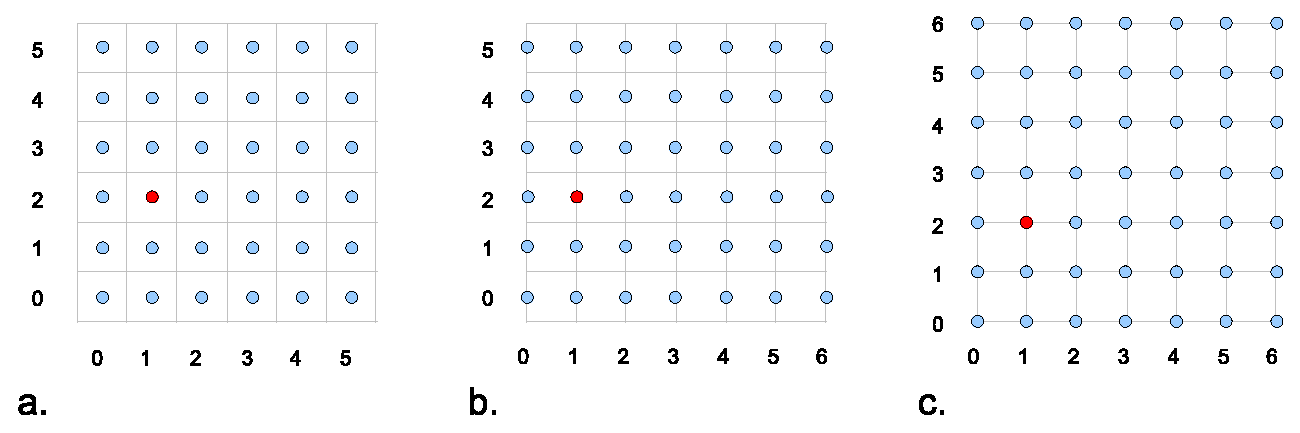
\includegraphics[width=6.5in]{\boxlibfigpath/data_loc2}
\caption[Data-centerings on the grid]
  {\label{fig:dataloc} Some of the different data-centerings:
  (a) cell-centered, (b) nodal in the $x$-direction, and (c) nodal in
  both the $x$- and $y$-directions.  Note that for nodal data, the
  integer index corresponds to the lower boundary in that direction.
  In each of these centerings, the red point has the same indices:\ (1,2).
  Not shown is the case where data is nodal in the $y$-direction only.}
\end{figure}

To simplify the description of the underlying AMR grid, BoxLib
provides a number of classes.  We briefly summarize some of the major
classes below.

First, note that when a Parallel application is compiled and linked,
the number of spatial dimensions (1,2 or 3), {\bf DIM},
 of the code must be specified.  The code that will be
built is specifically designed to run only with that number of dimensions.
(This is unlike the fParallel data structures in which we build
dimension-independent code at compile-time.)

\subsection{\IVtype}

\IVtype\ s are n-tuples of integers that are used to define
indices in space.    An example of an \IVtype\ in 2D would
be (3,5).

\subsection{\Boxtype}

A \Boxtype\ is simply a rectangular domain in space.  Note that \Boxtype\ s
do not hold any data themselves. A box basically contains
only the indices of its low end and high end as well as a type 
(cell-centered, edge-centered, or nodal).

\begin{figure}[h]
\centering
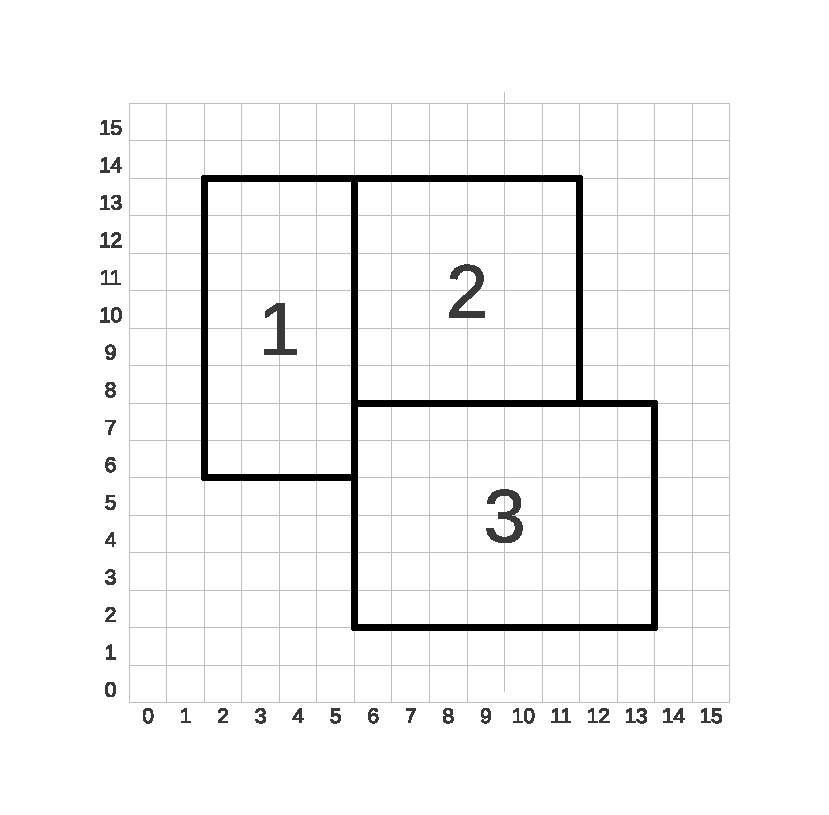
\includegraphics[width=4.0in]{\boxlibfigpath/index_grid2}
\caption[Single-level grid structure]
{\label{fig:boxes} Three boxes that comprise a single level.  At this
  resolution, the domain is 20$\times$18 zones.  Note that the
  indexing in BoxLib starts with $0$.}
\end{figure}

The computational domain is divided into boxes.  The collection of
boxes with the same resolution comprise a level.
Figure~\ref{fig:boxes} shows three boxes at the same level of
refinement.  The position of the boxes is with respect to a global
index space at that level.  For example, box 1 in the figure has 
{\tt lo} = (3,7) and {\tt hi} = (9,12).  

For a \Boxtype\ {\bf bx},
you can access the indices {\bf bx} using the 

\begin{itemize}
\item {\tt smallEnd}  -- for box 1 above this would return the \IVtype\ (3,7)
\item {\tt bigEnd} -- for box 1 above this would return the \IVtype\ (9,12)
\end{itemize}

\subsection{\BoxArray}

A \BoxArray\ is an array of boxes.   The size of the array is the 
number of boxes in the \BoxArray\ .

\subsection{{\tt FArrayBox}}

A \FAB\ (or {\tt FArrayBox}) is a ``Fortran Array Box'' that holds data.  It contains the
\Boxtype\ that it is built on as well as a pointer to the data 
that can be sent to a Fortran routine.
 
To build a \FAB\ you must specify the \Boxtype\ and the number of components.
For example, the section of code below builds a \FAB\ called {\tt myfab}
that has two components of data defined on the box from (0,0) to (31,15).

\begin{verbatim}
IntVect iv_lo(0,0);
IntVect iv_hi(31,15);
Box bx(iv_lo,iv_hi);
FArrayBox myfab;
myfab.define(bx,2);
\end{verbatim}

In Parallel, we don't usually deal with \FAB s alone, but rather
through \MultiFab s, described next.

\subsection{\MultiFab}

A \MultiFab\ is a collection of \FAB s at the same level of
refinement.  A \MultiFab\ is defined using a \BoxArray\ ,
number of components, and number of ``ghost'' calls that each box
will have.  Note that a \FAB\ has no concept of ghost cells, it
merely has a single box that identifies it.  A \MultiFab\ has
a "valid" region that is defined by the \BoxArray\ .  In addition,
each \FAB\ in the \MultiFab\ is built large enough to hold data
on the box associated with it {\it grown by ngrow ghost cells.}

If we had a \BoxArray\ , {\tt myba}, then we could define a \MultiFab\
as"

\begin{verbatim}
MultiFab mymf(myba,2,1);;
\end{verbatim}

This \MultiFab\ has two components of data and each \FAB\ in the \MultiFab\
contains ghost cells one row wide in all directions outside the box from the \BoxArray\ .

